% =====================================================================
%  THE LOSCHMIDT ECHO PROGRESSION
%  Spin-Echo Refocusing as the Empirical Completion of the
%  Resolution of Loschmidt's Paradox
%
%  Self-contained. Every technical term is defined in the text.
% =====================================================================
\documentclass[11pt,a4paper]{article}

\usepackage[utf8]{inputenc}
\usepackage[T1]{fontenc}
\usepackage{lmodern}
\usepackage[a4paper,margin=2.4cm]{geometry}
\usepackage{amsmath,amssymb,amsthm,mathtools}
\usepackage{bm}
\usepackage{booktabs}
\usepackage{array}
\usepackage{enumitem}
\usepackage{microtype}
\usepackage[round,sort&compress]{natbib}
\usepackage{tikz}
\usetikzlibrary{arrows.meta,decorations.pathmorphing}
\usepackage[colorlinks=true,linkcolor=blue!45!black,
            citecolor=blue!45!black,urlcolor=blue!45!black]{hyperref}

% ---- Theorem environments ----
\newtheoremstyle{thmstyle}{\topsep}{\topsep}{\itshape}{}{\bfseries}{.}{.5em}{}
\theoremstyle{thmstyle}
\newtheorem{theorem}{Theorem}[section]
\newtheorem{lemma}[theorem]{Lemma}
\newtheorem{proposition}[theorem]{Proposition}
\newtheorem{corollary}[theorem]{Corollary}
\theoremstyle{definition}
\newtheorem{definition}[theorem]{Definition}
\newtheorem{principle}[theorem]{Principle}
\newtheorem{example}[theorem]{Example}
\theoremstyle{remark}
\newtheorem{remark}[theorem]{Remark}

% ---- Shorthand ----
\newcommand{\R}{\mathbb{R}}
\newcommand{\N}{\mathbb{N}}
\newcommand{\Zp}{\mathbb{Z}^{+}}
\newcommand{\kB}{k_{\mathrm{B}}}
\newcommand{\Tprep}{T_{2}^{*}}
\newcommand{\Ttwo}{T_{2}}
\newcommand{\Mcount}{\mathcal{M}}
\newcommand{\Obs}{\mathcal{O}}
\newcommand{\Mic}{\mu}
\newcommand{\Count}{M}
\newcommand{\half}{\tfrac{1}{2}}
\newcommand{\Larmor}{\omega_{0}}

\title{\textbf{The Loschmidt Echo Progression:\\[2pt]
Spin-Echo Refocusing as the Empirical Completion\\
of the Resolution of Loschmidt's Paradox}}

\author{Kundai Farai Sachikonye\\
Technical University of Munich\\
Chair of Proteomics and Bioanalytics\\
\texttt{kundai.sachikonye@wzw.tum.de}}

\date{\today}

\begin{document}
\maketitle

% =====================================================================
\begin{abstract}
\noindent
Loschmidt's paradox (1876) asks how the manifest irreversibility of the
macroscopic world can be reconciled with the exact time-reversal
invariance of the underlying microscopic equations of motion. For a
century and a half the standard resolutions---Boltzmann's statistical
improbability, Gibbs's coarse-graining, the information-theoretic and
cosmological-boundary accounts, and environmental decoherence---have
shared a single presupposition: that time reversal is a well-defined,
in-principle-achievable operation whose macroscopic consequences merely
fail to be observed for contingent reasons. We argue that this
presupposition is empirically testable, that the experiment which tests
it already exists, and that it has been performed continuously since
1950 under the name of the \emph{nuclear spin echo}.

We proceed in two movements. First, we build from first principles an
operational account of physical time as a \emph{count of completed
oscillatory closures}, the \emph{partition count} $\Count$, and show
that this count obeys an exact identity $t=\Count/f$ with elapsed time,
is strictly monotone, and admits no operation that decrements it. The
central conceptual instrument is a rigorous separation of three
quantities that the paradox silently conflates: the macroscopic
\emph{observable} $\Obs$, the full \emph{microstate} $\Mic$, and the
partition count $\Count$. Second, we show that the spin echo is the
clean laboratory realisation of this separation. A refocusing
($180^{\circ}$) radio-frequency pulse recovers the observable
transverse magnetisation not by reversing the dynamics but by
re-placing, through a strictly forward operation, a configuration that
was never lost; the microstate is preserved throughout and the count
increases monotonically. We prove a \emph{Refocusability--Partition
Exclusion Theorem}: a dephasing contribution is recoverable by a pulse
if and only if it created no partition event, because a partition event
is precisely the commitment of the correlation one would need to undo
it. The irreversible residual---homogeneous transverse relaxation,
governed by $\Ttwo$---is therefore exactly the partition count made
measurable: the echo-amplitude deficit $e^{-2\tau/\Ttwo}$ is a
calibrated readout of accumulated, undeletable partition events.

We then exhibit the decisive empirical structure, the \emph{Loschmidt
echo progression}: a hierarchy of increasingly ambitious reversal
experiments---Hahn echo, Carr--Purcell--Meiboom--Gill pulse trains, and
genuine many-body Hamiltonian reversal (the magic echo and the
polarization/Loschmidt echo)---in which the more completely one
engineers the reversal, the more sharply an \emph{irreducible floor}
appears whose magnitude is set by the system's own internal dynamics
rather than by the residual imperfection of the engineering. The lab has
been running Loschmidt's own experiment for seventy years; every
refinement confirms the floor. We argue that this floor is a single
object viewed three ways, unifying the homogeneous-relaxation limit, the
non-decrementability of the partition count, and the positivity of the
smallest knowable error of any bounded observer. The completion of the
resolution is therefore not a stronger argument but an empirical fact:
the experiment named after Loschmidt refutes Loschmidt's premise.
\end{abstract}

\noindent\textbf{Keywords:} Loschmidt's paradox; irreversibility; arrow
of time; spin echo; Hahn echo; CPMG; Loschmidt echo; transverse
relaxation; $T_2$ and $T_2^{*}$; time-reversal invariance; partition
count; second law of thermodynamics.

\tableofcontents

% =====================================================================
\section{Introduction}
\label{sec:intro}
% =====================================================================

\subsection{The paradox}
\label{sec:the-paradox}

In 1876, Josef Loschmidt raised an objection to Ludwig Boltzmann's
program of deriving the second law of thermodynamics from the mechanics
of atoms \citep{loschmidt1876}. The objection is disarmingly simple. The
microscopic equations of motion governing a system of particles---in
Loschmidt's day, Newton's laws; in their canonical form, Hamilton's
equations---possess a symmetry: if one takes any solution of the
equations and reverses the sign of time while simultaneously reversing
all velocities, the result is again a solution. The equations cannot
distinguish the future from the past; they are, in the technical sense
made precise in Section~\ref{sec:time-reversal}, \emph{time-reversal
invariant}.

Yet the macroscopic world is flagrantly asymmetric in time. Heat flows
from hot to cold and never the reverse; a drop of ink disperses through
water and never spontaneously reassembles; an egg breaks but is never
seen to unbreak. The second law of thermodynamics codifies this: the
entropy of an isolated system does not decrease. Loschmidt's challenge
was this: if the microscopic laws are indifferent to the direction of
time, from where does the macroscopic arrow arise? More pointedly: take
a gas that has expanded irreversibly to fill its container, and at some
instant reverse every molecular velocity. The reversed state is a
perfectly legitimate solution of the same equations, and it will
retrace the expansion backwards, the gas re-collecting itself into the
corner it came from, entropy decreasing. The laws permit it. Why do we
never see it?

\subsection{Why the paradox has resisted resolution}
\label{sec:why-resisted}

Boltzmann's reply \citep{boltzmann1877} was statistical: the reversed
evolution is not impossible, merely overwhelmingly improbable. The
number of microscopic configurations corresponding to a dispersed,
high-entropy macrostate vastly exceeds the number corresponding to a
concentrated, low-entropy one; an evolution that decreases entropy
requires the system to be launched from one of the astronomically rare
``conspiratorial'' states, and such states are never prepared in
practice. The probability of spontaneous entropy decrease in a
macroscopic body is of order $e^{-\Delta S/\kB}$, with $\Delta S/\kB$ of
order $10^{23}$; the recurrence and reversal times exceed the age of the
universe by factors that defeat description.

This statistical resolution, refined over a century by Gibbs's
coarse-graining \citep{gibbs1902}, the information-theoretic
reformulation \citep{jaynes1957}, the cosmological-boundary account
\citep{penrose1989,penrose2004}, the dissipative-structures program
\citep{prigogine1980}, and environmental decoherence
\citep{zurek2003}, has become orthodoxy. We will review these in
Section~\ref{sec:standard}. They differ in emphasis but share a single
structural commitment, which we will call the \emph{reversibility
presupposition}:

\begin{quote}
\emph{Time reversal is a well-defined operation. It is in principle
achievable; the reversed trajectories exist and are physically
realisable; macroscopic irreversibility is the statement that we do not,
for contingent reasons (improbability, ignorance, openness, special
initial conditions), happen to realise them.}
\end{quote}

Every standard resolution accepts Loschmidt's framing and then explains
why the reversed evolutions, though available, are not seen. None asks
whether the operation Loschmidt invoked---``reverse all the
velocities''---is a coherent physical operation at all, or whether, when
one attempts to perform it, anything answering to ``running the dynamics
backwards'' actually occurs.

\subsection{The missing empirical witness}
\label{sec:missing-witness}

There is a tradition of treating Loschmidt's velocity reversal as a
thought experiment---a \emph{Gedankenexperiment} forever beyond the
reach of the laboratory, since one cannot grab $10^{23}$ molecules and
flip their momenta. This is a mistake. A close and informative
laboratory cousin of Loschmidt's operation has been performed routinely
since 1950, in essentially every nuclear magnetic resonance laboratory
on Earth, under the name of the \emph{spin echo} \citep{hahn1950}.

In a spin-echo experiment an ensemble of nuclear spins is prepared in a
coherent transverse state, allowed to ``dephase'' (lose macroscopic
coherence) under the action of a distribution of precession frequencies,
and then subjected to a single radio-frequency pulse---the
\emph{refocusing} or $180^{\circ}$ pulse---after which the ensemble
spontaneously \emph{rephases}, the macroscopic signal reappearing as an
``echo.'' To the eye, the dephasing is undone, coherence is restored,
and the entropy of the spin system decreases. The refocusing pulse looks
exactly like a controlled, partial realisation of Loschmidt's velocity
reversal: it inverts the accumulated phases and the system retraces its
loss of coherence.

If the spin echo were what it superficially appears to be---a small,
controlled time reversal---it would be evidence that Loschmidt's
operation is coherent and approximable, and that the only barrier to
full reversal is the practical one of scale. We will argue that the spin
echo is \emph{not} what it appears to be, and that understanding
precisely what it is supplies the missing piece in the resolution of the
paradox. The spin echo is not a partial reversal of the dynamics; it is
a clean physical separation of two things the dynamics keeps distinct
and the paradox keeps conflated. And the family of experiments it
anchors---the \emph{Loschmidt echo progression} of
Section~\ref{sec:progression}---constitutes a seventy-year experimental
test of the reversibility presupposition itself, with a definite and
repeatedly confirmed outcome.

\subsection{Thesis and contributions}
\label{sec:thesis}

Our thesis is that the spin echo \emph{completes} the resolution of
Loschmidt's paradox by converting a conceptual claim into an empirical
one. The conceptual claim, developed in
Sections~\ref{sec:partition}--\ref{sec:three-quantities}, is that time
is constituted by an irreducibly monotone count and that ``reversing the
dynamics'' is a category error---a confusion of a transformation of
mathematical solutions with an operation on physical systems. The
empirical claim, developed in
Sections~\ref{sec:nmr}--\ref{sec:progression}, is that when one builds
the best available physical approximation to Loschmidt's operation and
makes it progressively better, what one measures is not progressively
better reversal but the progressively sharper exposure of an irreducible
floor.

The specific contributions are:

\begin{enumerate}[leftmargin=1.4em,itemsep=0.25em]
\item \textbf{A from-scratch operational account of time as a partition
count} (Section~\ref{sec:partition}), with the Time--Count Identity
$t=\Count/f$ derived non-circularly, the strict monotonicity of the
count, and the incoherence of any operation that would decrement it.

\item \textbf{The Three-Quantity Separation}
(Section~\ref{sec:three-quantities}): a precise distinction between the
macroscopic observable $\Obs$, the microstate $\Mic$, and the partition
count $\Count$, together with the claim that Loschmidt's intuition rests
on conflating them.

\item \textbf{A complete, self-contained account of the nuclear spin
echo} (Section~\ref{sec:nmr}), defining every term---magnetisation,
Larmor precession, the rotating frame, radio-frequency pulses, free
induction decay, and the two distinct transverse-relaxation times
$\Tprep$ and $\Ttwo$---so that the argument is legible to a reader with
no background in magnetic resonance.

\item \textbf{The Echo-Configuration Recovery Theorem}
(Section~\ref{sec:configuration}): the echo recovers the observable by a
forward operation on a preserved microstate, while the count advances
monotonically.

\item \textbf{The Refocusability--Partition Exclusion Theorem}
(Section~\ref{sec:exclusion}): a dephasing contribution is refocusable
if and only if it created no partition event. This is the structural
lock that explains \emph{why} the reversible and irreversible parts of
relaxation are exactly the configurational and the count-incrementing
parts.

\item \textbf{The Echo-Deficit Identity}
(Section~\ref{sec:deficit}): the homogeneous relaxation envelope
$e^{-2\tau/\Ttwo}$ is a calibrated, directly observed measurement of
accumulated partition events---the count made visible.

\item \textbf{The Loschmidt echo progression and the irreducible floor}
(Section~\ref{sec:progression}): a hierarchy of reversal experiments in
which improved engineering exposes an engineering-independent floor, and
an argument that this floor is a single object unifying the
homogeneous-relaxation limit, the non-decrementability of the count, and
the positive smallest knowable error of any bounded observer
(Section~\ref{sec:floor-unification}).
\end{enumerate}

\subsection{Structure of the paper}
\label{sec:structure}

Section~\ref{sec:loschmidt-precise} states the paradox in precise
mathematical form and reviews the standard resolutions and their common
presupposition. Section~\ref{sec:partition} develops the partition-count
account of time from first principles.
Section~\ref{sec:three-quantities} establishes the Three-Quantity
Separation. Section~\ref{sec:nmr} is a complete primer on the physics of
the spin echo. Sections~\ref{sec:configuration}, \ref{sec:exclusion},
and \ref{sec:deficit} prove the three core theorems.
Section~\ref{sec:progression} presents the experimental hierarchy.
Section~\ref{sec:floor-unification} states the floor unification.
Section~\ref{sec:resolution} assembles the completed resolution.
Section~\ref{sec:objections} addresses objections;
Section~\ref{sec:predictions} states falsifiable predictions;
Section~\ref{sec:discussion} discusses connections to measurement,
computation, and quantum chaos; Section~\ref{sec:conclusion} concludes.

% =====================================================================
\section{Loschmidt's Paradox in Precise Form}
\label{sec:loschmidt-precise}
% =====================================================================

\subsection{Hamiltonian dynamics}
\label{sec:hamiltonian}

We begin with the mathematical setting, defining each object as we go.

A classical mechanical system of $N$ point particles is described by
specifying, at each instant, the position and momentum of every
particle. The collection of all positions is written
$q=(q_{1},\dots,q_{3N})$ and the collection of all momenta
$p=(p_{1},\dots,p_{3N})$; here each $q_{i}$ and $p_{i}$ is a real number,
and the factor $3N$ counts the three spatial directions for each of the
$N$ particles. The pair $(q,p)$ is a single point in a $6N$-dimensional
space called \emph{phase space}, denoted $\Gamma$. A point of $\Gamma$
is a complete instantaneous specification of the mechanical system; we
call it a \emph{microstate}.

The dynamics is generated by a single function $H(q,p)$, the
\emph{Hamiltonian}, which for our purposes equals the total energy
expressed in terms of positions and momenta. The time evolution of the
microstate is given by \emph{Hamilton's equations},
\begin{equation}
\dot{q}_{i} = \frac{\partial H}{\partial p_{i}}, \qquad
\dot{p}_{i} = -\frac{\partial H}{\partial q_{i}},
\label{eq:hamilton}
\end{equation}
where the overdot denotes the derivative with respect to time $t$ and
$\partial/\partial q_{i}$, $\partial/\partial p_{i}$ denote partial
derivatives. Given an initial microstate $(q(0),p(0))$,
Equations~\eqref{eq:hamilton} determine the microstate $(q(t),p(t))$ at
all later (and earlier) times. The map sending the initial microstate to
the microstate at time $t$ is called the \emph{Hamiltonian flow} and
written $\varphi_{t}:\Gamma\to\Gamma$. The flow is deterministic and
invertible: $\varphi_{t}$ has inverse $\varphi_{-t}$.

\subsection{Time-reversal invariance}
\label{sec:time-reversal}

Define the \emph{time-reversal map} $R:\Gamma\to\Gamma$ by
$R(q,p)=(q,-p)$: it leaves positions unchanged and flips the sign of all
momenta. For the broad and physically central class of Hamiltonians that
are even in the momenta---$H(q,-p)=H(q,p)$, which holds whenever the
kinetic energy is quadratic in $p$ and the forces derive from a
position-dependent potential---one verifies directly from
\eqref{eq:hamilton} that
\begin{equation}
\varphi_{-t} = R \circ \varphi_{t} \circ R .
\label{eq:trinv}
\end{equation}
In words: evolving forward for time $t$, flipping the momenta, evolving
forward again for time $t$, and flipping the momenta once more returns
the system to its starting microstate. Equivalently, if $(q(t),p(t))$ is
a solution of Hamilton's equations, then $(q(-t),-p(-t))$ is also a
solution. This is what it means for the dynamics to be
\emph{time-reversal invariant}: the set of solutions is mapped onto
itself by the combined operation of reversing time and flipping momenta.
It is a property of the \emph{solution set} of the equations.

\begin{remark}[The hinge of the whole problem]
\label{rem:hinge}
Equation~\eqref{eq:trinv} is a statement about \emph{mathematical
solutions}. It says that a certain transformation carries one solution
of the equations to another solution. It does not say---and this
distinction is the hinge on which the entire paradox turns---that there
exists a \emph{physical operation}, performable in a laboratory, whose
execution carries a physical system from the first solution to the
second. We will return to this in
Sections~\ref{sec:three-quantities} and \ref{sec:resolution}.
\end{remark}

\subsection{Liouville's theorem and Poincar\'e recurrence}
\label{sec:liouville-poincare}

Two classical results constrain the flow and sharpen the paradox.

\emph{Liouville's theorem} \citep{liouville1838} states that the
Hamiltonian flow preserves phase-space volume: if one takes any region
$A\subseteq\Gamma$ of volume $\mathrm{vol}(A)$ and lets every point of it
evolve for time $t$, the resulting region $\varphi_{t}(A)$ has the same
volume, $\mathrm{vol}(\varphi_{t}(A))=\mathrm{vol}(A)$. The flow stirs
phase space without compressing or expanding it, like an
incompressible fluid. A consequence is that the flow cannot have
attractors: it cannot funnel a fat region of initial conditions down to
a thin set of final ones. Whatever irreversibility we observe cannot be
a contraction of phase-space volume.

\emph{Poincar\'e's recurrence theorem} \citep{poincare1890} states that
if the accessible phase space has finite volume (as it does for a system
of bounded energy confined to a bounded region), then almost every
microstate returns arbitrarily close to its initial value, infinitely
often, given enough time. Ernst Zermelo \citep{zermelo1896} wielded this
against Boltzmann: if every state recurs, no quantity can increase
monotonically forever, and the second law cannot hold strictly.
Boltzmann's reply \citep{boltzmann1896} was again statistical---the
recurrence times for macroscopic systems are so vast as to be physically
irrelevant. We record recurrence here because, as we shall see in
Section~\ref{sec:three-quantities}, the partition account dissolves the
Zermelo objection at a different level: a recurrence of the
\emph{microstate} is not a recurrence of the \emph{count}, and it is the
count, not the microstate, that constitutes elapsed time.

\subsection{The reversibility objection, sharply}
\label{sec:objection-sharp}

We can now state Loschmidt's objection in its sharpest form. Consider a
gas prepared at $t=0$ in a low-entropy macrostate (all molecules in one
corner) and evolved to time $T$, by which point it has spread to fill its
container (a high-entropy macrostate). Apply the time-reversal map $R$ to
the microstate at $T$: flip all the momenta. By
Equation~\eqref{eq:trinv}, the subsequent forward evolution
$\varphi_{t}$ for $0\le t\le T$ carries the system back through the
positions it occupied during the expansion, in reverse order, until at
time $2T$ it sits again in the corner. Entropy will have decreased. The
trajectory is a bona fide solution of the same equations that governed
the expansion. The objection is: \emph{the laws sanction this; the
second law forbids it; how can both be true?}

\subsection{The standard resolutions and their common structure}
\label{sec:standard}

We summarise the orthodox answers and exhibit their shared
presupposition. Table~\ref{tab:standard} collects them.

\begin{table*}[t]
\centering
\small
\caption{Standard resolutions of Loschmidt's paradox. Each accepts that
time reversal is a coherent, in-principle-achievable operation and
explains why its consequences are not observed.}
\label{tab:standard}
\begin{tabular}{p{0.20\textwidth}p{0.40\textwidth}p{0.32\textwidth}}
\toprule
\textbf{Resolution} & \textbf{Account of why reversal is not seen} &
\textbf{Residual commitment} \\
\midrule
Boltzmann statistical \citep{boltzmann1877} &
Reversed trajectories require astronomically improbable initial
microstates ($P\sim e^{-\Delta S/\kB}$). &
Reversal is possible, merely improbable; leaves open ``with enough luck
or control.'' \\
\addlinespace
Gibbs coarse-graining \citep{gibbs1902} &
Entropy increases only for a coarse-grained (smeared) distribution;
fine-grained entropy is constant by Liouville. &
Irreversibility is observer-relative; different coarse-grainings give
different entropies. \\
\addlinespace
Information-theoretic \citep{jaynes1957} &
Entropy measures the observer's ignorance of the microstate; it grows
because we track fewer degrees of freedom. &
Irreversibility is epistemic; the underlying reversal remains coherent.
\\
\addlinespace
Cosmological boundary \citep{penrose1989,penrose2004} &
The arrow stems from an exceptionally low-entropy initial state of the
universe. &
Explains the global gradient, not the absence of local reversal events.
\\
\addlinespace
Decoherence \citep{zurek2003} &
Entanglement with an uncontrolled environment destroys the phase
relations reversal would require. &
Applies to open systems; the closed-system reversal is granted as
coherent. \\
\bottomrule
\end{tabular}
\end{table*}

Each entry of Table~\ref{tab:standard} is correct within its domain.
What they share is the residual commitment in the third column: the
\emph{operation} of time reversal is treated as meaningful and
realisable, and only its \emph{consequences} are explained away. The
present paper attacks the commitment itself, and---crucially---does so
in a way that is decided not by argument but by an experiment that has
been running since 1950.

% =====================================================================
\section{Time as a Partition Count}
\label{sec:partition}
% =====================================================================

We now build, from first principles and without reference to any prior
framework, the conceptual apparatus we need: an operational account of
what physical time \emph{is}, in which the asymmetry we seek is not
imposed but constitutive.

\subsection{Time is read from a counter}
\label{sec:time-counter}

Ask how elapsed time is established in any actual physical measurement.
The answer is always the same: one counts the cycles of a reference
oscillator. A pendulum clock counts swings; a quartz watch counts
crystal vibrations; the international definition of the second counts a
fixed number---$9{,}192{,}631{,}770$---of oscillations of the radiation
associated with a hyperfine transition of the caesium-133 atom
\citep{essen1955}. In every case the procedure is identical: fix a
reference oscillator, count its completed cycles, and report the count
(suitably scaled) as the elapsed time.

We take this literally. Time, as an operationally defined physical
quantity, \emph{is} a count of completed oscillatory cycles. We make this
precise.

\begin{definition}[Oscillatory closure]
\label{def:closure}
Let a system possess a degree of freedom describable by an angle
$\theta$ taking values on the circle $[0,2\pi)$. An \emph{oscillatory
closure} is the event of $\theta$ completing one full traversal of
$[0,2\pi)$ and returning to its starting value. A closure is a purely
topological event---the completion of a loop in configuration
space---and its occurrence makes no reference to any unit of duration.
\end{definition}

\begin{definition}[Partition count]
\label{def:count}
The \emph{partition count} $\Count(t)\in\Zp$ of a system relative to a
reference oscillator is the integer number of oscillatory closures of
that oscillator completed up to time $t$. The term ``partition'' records
that each closure partitions the system's history into a
before and an after: the closure is the irreducible unit by which one
stretch of existence is marked off from the next.
\end{definition}

\begin{remark}[Non-circularity]
\label{rem:noncircular}
One might object that a ``cycle'' already presupposes a duration, making
the definition circular. It does not. A closure is defined by the
angular condition ``$\theta$ has traversed $[0,2\pi)$ and returned,''
which is a statement about the geometry of the trajectory in
configuration space, not about how long the traversal took. Two
oscillators are compared by the dimensionless ratio of their counts,
$\Count_{A}/\Count_{B}$; one of them is promoted to the standard, and a
unit of duration is \emph{defined} by stipulating how many of its
closures constitute that unit (for the SI second, $9{,}192{,}631{,}770$
closures of the caesium standard). Frequency in hertz is then the ratio
of a system's count to the caesium count. Duration and frequency are
\emph{derived} from counting; counting does not presuppose them.
\end{remark}

\subsection{Bounded systems oscillate}
\label{sec:bounded-osc}

The partition count is well defined whenever there is an oscillator to
count, and bounded physical systems always supply one.

\begin{proposition}[Oscillatory necessity]
\label{prop:osc-necessity}
A mechanical system confined to a region of finite spatial extent and
possessing finite energy executes bounded motion; on any such bounded
energy surface, no coordinate can escape monotonically to infinity, and
(in the absence of fixed points, which are excluded for systems at
positive temperature) the motion is oscillatory: every trajectory
returns repeatedly to the neighbourhood of its prior configurations.
\end{proposition}

\begin{proof}[Sketch]
Confinement to a bounded region with finite energy means the accessible
phase space is bounded, hence (being also closed) compact and of finite
volume. A coordinate escaping monotonically would leave every bounded
region, contradicting confinement. By Poincar\'e recurrence
(Section~\ref{sec:liouville-poincare}) almost every trajectory returns
arbitrarily near its initial condition; combined with the absence of
fixed points this forces the recurrent returns to be traversed
cyclically, i.e.\ oscillatorily.
\end{proof}

Proposition~\ref{prop:osc-necessity} guarantees that the count of
Definition~\ref{def:count} is available for any bounded system, and in
particular for the trapped nuclear spins of Section~\ref{sec:nmr}.

\subsection{The Time--Count Identity}
\label{sec:time-count}

\begin{theorem}[Time--Count Identity]
\label{thm:time-count}
For a reference oscillator of frequency $f$ (defined, per
Remark~\ref{rem:noncircular}, as the number of its closures per unit of
the standard), the partition count and the elapsed time satisfy
\begin{equation}
\Count(t) = f\,t, \qquad\text{equivalently}\qquad t = \frac{\Count}{f},
\label{eq:tmf}
\end{equation}
exactly, and the rate of counting equals the frequency,
$\mathrm{d}\Count/\mathrm{d}t=f$.
\end{theorem}

\begin{proof}
By definition of frequency the oscillator completes $f$ closures per unit
of standard time; in elapsed time $t$ it completes $ft$ closures, which
is the count by Definition~\ref{def:count}. The relation
$\mathrm{d}\Count/\mathrm{d}t=f$ is the differential form of the same
statement. The continuous-time parameter $t\in\R$ of the formalism is the
$f\to\infty$ idealisation of the integer count, in which the discrete
steps become unresolvably fine.
\end{proof}

Read from right to left, Equation~\eqref{eq:tmf} would be circular
($f$ presupposes $t$); read as the definition of the derived continuous
parameter $t$ in terms of the primitive count $\Count$, it is not. The
identity records that the count \emph{is} the time, in units fixed by the
choice of standard.

\subsection{Monotonicity and the incoherence of decrement}
\label{sec:monotone}

\begin{theorem}[Strict monotonicity]
\label{thm:monotone}
The partition count is strictly increasing along any physical evolution:
if $t_{2}>t_{1}$ and at least one closure occurs in $[t_{1},t_{2}]$, then
$\Count(t_{2})>\Count(t_{1})$.
\end{theorem}

\begin{proof}
By Theorem~\ref{thm:time-count}, $\Count(t_{2})-\Count(t_{1})=f(t_{2}-t_{1})>0$.
\end{proof}

\begin{theorem}[Incoherence of decrement]
\label{thm:incoherence}
No physical operation can decrease the partition count. In particular,
the mathematical time-reversal map $R$ of Section~\ref{sec:time-reversal}
has no realisation as a count-decrementing operation.
\end{theorem}

\begin{proof}
Suppose an operation $\Obs^{*}$ purported to take the count from
$\Count$ to $\Count-k$ with $k>0$. Its execution is itself a physical
process occupying a positive interval $\Delta t>0$, during which, by
Theorem~\ref{thm:monotone}, the reference oscillator completes at least
$f\,\Delta t>0$ closures. The count after the operation therefore exceeds
the count before it by at least $f\,\Delta t$, contradicting the
supposition that it decreased. The map $R$ acts on the solution set of
the equations (Section~\ref{sec:time-reversal}); applying it is an act of
mathematical substitution, not a laboratory procedure, and so it does not
act on $\Count$ at all. There is no operation whose execution decrements
the count, because executing anything increments it.
\end{proof}

Theorem~\ref{thm:incoherence} is the partition-level statement of the
arrow of time: not that decrement is improbable, but that the very
attempt to perform a decrementing operation is a counting process, hence
incrementing. The second law, in this reading, is not a statistical
tendency layered on reversible foundations; it is the observation that
the count cannot decrease because counting is what time is.

% =====================================================================
\section{The Three-Quantity Separation}
\label{sec:three-quantities}
% =====================================================================

The conceptual core of the paper is the recognition that Loschmidt's
intuition---``if the trajectory can be retraced, the system returns to
its past''---silently identifies three quantities that must be kept
distinct. We name them and state their relations; the spin echo of
Section~\ref{sec:nmr} will make the distinctions visible and measurable.

\begin{definition}[The three quantities]
\label{def:three}
For a system of many constituents we distinguish:
\begin{enumerate}[leftmargin=1.6em,label=(\roman*),itemsep=0.2em]
\item the \emph{microstate} $\Mic(t)$: the complete instantaneous
specification of every constituent (for the gas, the full point of phase
space; for the spins of Section~\ref{sec:nmr}, the full list of
individual spin phases);
\item the \emph{observable} $\Obs(t)$: a coarse, macroscopically
accessible function of the microstate (for the gas, the spatial density
profile; for the spins, the net transverse magnetisation), in general
many-to-one, so that many microstates share one observable value;
\item the \emph{partition count} $\Count(t)$: the monotone count of
Section~\ref{sec:partition}, recording how much has happened.
\end{enumerate}
\end{definition}

\begin{principle}[The conflation]
\label{prin:conflation}
Loschmidt's reversibility intuition rests on the implicit identification
$\Obs\equiv\Mic\equiv\Count$: that recovering the observable
($\Obs(2T)=\Obs(0)$) is the same as restoring the microstate
($\Mic(2T)=\Mic(0)$), which is the same as returning to the past
($\Count(2T)=\Count(0)$). The three are distinct, and conflating them is
what makes ``the trajectory returned'' sound like ``the system went
back.''
\end{principle}

\begin{theorem}[Genuine distinctness]
\label{thm:distinct}
The three quantities of Definition~\ref{def:three} are logically
independent in the following sense. (i) $\Obs$ may return to a past value
while $\Mic$ does not: many microstates share an observable, so
$\Obs(t_{2})=\Obs(t_{1})$ does not imply $\Mic(t_{2})=\Mic(t_{1})$. (ii)
$\Mic$ may return to a past value while $\Count$ does not: a Poincar\'e
recurrence restores the microstate but, by Theorem~\ref{thm:monotone},
the count has strictly increased. (iii) $\Count$ never returns to a past
value at all (Theorem~\ref{thm:incoherence}).
\end{theorem}

\begin{proof}
(i) is the many-to-one character of $\Obs$ in
Definition~\ref{def:three}(ii). (ii): at a recurrence time $t_{2}$ with
$\Mic(t_{2})\approx\Mic(t_{1})$, Theorem~\ref{thm:monotone} gives
$\Count(t_{2})>\Count(t_{1})$ because closures accumulated in the
interim. (iii) is Theorem~\ref{thm:incoherence}.
\end{proof}

Theorem~\ref{thm:distinct} already dissolves the Zermelo recurrence
objection (Section~\ref{sec:liouville-poincare}) at the level of
principle: a recurrence is a return of $\Mic$, not of $\Count$, and it is
$\Count$ that constitutes elapsed time. But a principle is not an
experiment. The remainder of the paper shows that the spin echo realises
this separation in the laboratory---and, in the Loschmidt echo
progression, measures the separating quantity directly.

% =====================================================================
\section{The Nuclear Spin Echo: A Complete Account}
\label{sec:nmr}
% =====================================================================

This section is a self-contained primer. A reader who knows magnetic
resonance may skim it; a reader who does not will find every term used in
the theorems defined here.

\subsection{Spins, magnetic moments, and the Larmor precession}
\label{sec:larmor}

Many atomic nuclei possess an intrinsic angular momentum called
\emph{spin}, and with it a \emph{magnetic moment}: the nucleus behaves
like a tiny bar magnet whose orientation is tied to the spin. Write the
magnetic moment of a single nucleus as a vector $\bm{\mu}$. The
proportionality between moment and spin angular momentum is the
\emph{gyromagnetic ratio} $\gamma$, a constant characteristic of the
nuclear species.

Place the nucleus in a strong, uniform, static magnetic field $\bm{B}_0$
pointing along the laboratory $z$-axis. A magnetic moment in a field
experiences a torque that, rather than simply aligning it, causes it to
\emph{precess}---to sweep out a cone around the field direction, like a
spinning top leaning in gravity. The angular frequency of this precession
is the \emph{Larmor frequency}
\begin{equation}
\Larmor = \gamma B_{0}.
\label{eq:larmor}
\end{equation}
A nucleus whose local field is $B$ precesses at $\gamma B$; we will see
that small variations in the local field across the sample are the source
of everything that follows.

For an ensemble of many identical nuclei (say, the hydrogen nuclei in a
millilitre of water, of order $10^{22}$ of them), the individual moments
sum to a macroscopic \emph{magnetisation} vector $\bm{M}$. In thermal
equilibrium $\bm{M}$ points along $\bm{B}_0$ (along $z$): there is a
slight excess of moments aligned with the field, and their vector sum is
a net longitudinal magnetisation $M_{z}$. The transverse components
($M_{x}$, $M_{y}$) vanish in equilibrium because the individual moments
are uniformly distributed around the precession cone---their phases are
random, and the transverse components cancel.

\subsection{The rotating frame}
\label{sec:rotating-frame}

It is convenient to describe the motion in a coordinate frame that
rotates about the $z$-axis at the Larmor frequency $\Larmor$. In this
\emph{rotating frame}, a moment precessing exactly at $\Larmor$ appears
stationary; a moment precessing at a slightly different frequency
$\Larmor+\Delta\omega$ appears to rotate slowly at the \emph{offset}
$\Delta\omega$. The rotating frame removes the rapid common precession and
leaves visible only the differences that matter. Throughout, ``phase''
$\varphi$ means the angle of a moment's transverse component in the
rotating frame.

\subsection{Radio-frequency pulses}
\label{sec:rf-pulses}

A short burst of oscillating magnetic field, applied perpendicular to
$\bm{B}_0$ and tuned to the Larmor frequency, exerts a controllable
torque on the magnetisation. In the rotating frame this \emph{radio
frequency (RF) pulse} appears as a steady field about which the
magnetisation rotates; by choosing the burst's duration and amplitude one
rotates $\bm{M}$ by any desired angle. Two pulses concern us:

\begin{itemize}[leftmargin=1.4em,itemsep=0.2em]
\item the \emph{$90^{\circ}$ pulse} (or $\pi/2$ pulse), which tips the
equilibrium magnetisation from the $z$-axis into the transverse
($xy$) plane, creating a coherent transverse magnetisation in which all
moments start with the same phase;
\item the \emph{$180^{\circ}$ pulse} (or $\pi$ pulse, the
\emph{refocusing} pulse), which rotates the magnetisation by half a turn
about an axis in the transverse plane, with the effect---central to the
echo---of replacing each moment's phase $\varphi$ by $-\varphi$.
\end{itemize}

\subsection{Free induction decay and the two dephasings}
\label{sec:fid}

Apply a $90^{\circ}$ pulse at $t=0$. The magnetisation now lies in the
transverse plane, all moments in phase, producing a maximal transverse
signal---a precessing magnetisation induces an oscillating voltage in a
nearby pickup coil, and this voltage is what the spectrometer records.

Immediately the signal begins to decay. The decay, called the \emph{free
induction decay} (FID), happens because the moments do not all precess at
exactly the same frequency, and so their phases spread out, or
\emph{dephase}: the moments fan out around the transverse plane and their
vector sum---the observable transverse magnetisation---shrinks. There are
two physically distinct causes of dephasing, and the entire argument of
this paper hinges on telling them apart.

\paragraph{Inhomogeneous dephasing ($\Tprep$).} The static field $\bm{B}_0$
is never perfectly uniform across a real sample, and different nuclei sit
in slightly different chemical environments. A nucleus at a location where
the field is $B_{0}+\delta B_{i}$ precesses at offset
$\Delta\omega_{i}=\gamma\,\delta B_{i}$ in the rotating frame. These
offsets are \emph{static}: each nucleus keeps its own fixed offset for
the duration of the experiment. The phase it accumulates is therefore the
exactly determined quantity
\begin{equation}
\varphi_{i}^{\mathrm{stat}}(t) = \Delta\omega_{i}\,t .
\label{eq:phistat}
\end{equation}
The spread of fixed offsets makes the ensemble fan out and the signal
decay, on a timescale denoted $\Tprep$ (``T-two-star''). This dephasing
is \emph{deterministic} and, as we will see, \emph{reversible}.

\paragraph{Homogeneous dephasing ($\Ttwo$).} Superimposed on the static
offsets are \emph{fluctuating} local fields: each nucleus is jostled by
the time-varying magnetic fields of its neighbours (spin--spin
interactions), by molecular tumbling, and by diffusion through field
gradients \citep{bloch1946,bpp1948}. The instantaneous offset of nucleus
$i$ thus has a randomly varying part $\delta\omega_{i}(t)$ with some short
correlation time, and the phase it accumulates from this part,
\begin{equation}
\varphi_{i}^{\mathrm{fluc}}(t) = \int_{0}^{t}\delta\omega_{i}(t')\,
\mathrm{d}t',
\label{eq:phifluc}
\end{equation}
is a stochastic quantity. This dephasing proceeds on a timescale
$\Ttwo$ (``T-two''), the \emph{true} or \emph{homogeneous} transverse
relaxation time. It is \emph{stochastic} and, as we will see,
\emph{irreversible}.

The two timescales combine, for the observable FID envelope, as
\begin{equation}
\frac{1}{\Tprep} = \frac{1}{\Ttwo} + \frac{1}{\Ttwo^{\mathrm{inh}}},
\qquad \Tprep \le \Ttwo ,
\label{eq:t2star}
\end{equation}
where $1/\Ttwo^{\mathrm{inh}}$ is the contribution of the static
inhomogeneity. Because the inhomogeneous part is usually the larger, the
raw FID decays \emph{faster} ($\Tprep$) than the true relaxation
($\Ttwo$) would dictate. The spin echo is the device that strips away the
inhomogeneous part and reveals $\Ttwo$.

\subsection{The Hahn echo}
\label{sec:hahn}

Erwin Hahn's 1950 discovery \citep{hahn1950} is the following sequence,
sketched in Figure~\ref{fig:pulse}:

\begin{enumerate}[leftmargin=1.5em,itemsep=0.15em]
\item At $t=0$, a $90^{\circ}$ pulse creates coherent transverse
magnetisation; the FID begins and the ensemble dephases.
\item At $t=\tau$, a $180^{\circ}$ pulse replaces every phase
$\varphi_{i}(\tau)$ by $-\varphi_{i}(\tau)$.
\item The ensemble continues to precess under the \emph{same} field as
before.
\item At $t=2\tau$, the signal spontaneously reappears as an
\emph{echo}.
\end{enumerate}

\begin{figure}[t]
\centering
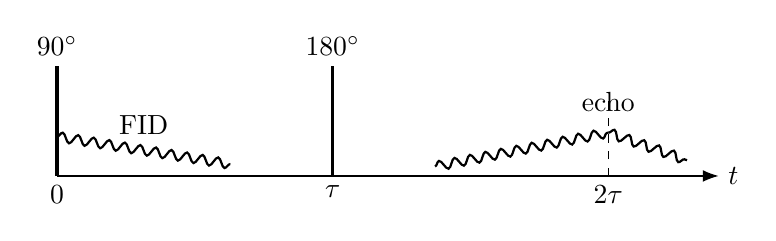
\begin{tikzpicture}[scale=1.0]
% time axis
\draw[-{Latex[length=2mm]}] (0,0) -- (8.4,0) node[right]{$t$};
% pulses
\draw[very thick] (0,0) -- (0,1.4); \node[above] at (0,1.4){$90^{\circ}$};
\draw[very thick] (3.5,0) -- (3.5,1.4); \node[above] at (3.5,1.4){$180^{\circ}$};
% labels for times
\node[below] at (0,0){$0$};
\node[below] at (3.5,0){$\tau$};
\node[below] at (7.0,0){$2\tau$};
\draw[dashed] (7.0,0) -- (7.0,1.0);
% FID envelope (decaying) after 0
\draw[thick,decorate,decoration={snake,amplitude=0.6mm,segment length=2mm}]
   (0,0.5) -- (2.2,0.15);
% growing echo before 2tau and decaying after
\draw[thick,decorate,decoration={snake,amplitude=0.6mm,segment length=2mm}]
   (4.8,0.12) -- (7.0,0.55);
\draw[thick,decorate,decoration={snake,amplitude=0.6mm,segment length=2mm}]
   (7.0,0.55) -- (8.0,0.2);
\node[above] at (7.0,0.7){echo};
\node at (1.1,0.65){FID};
\end{tikzpicture}
\caption{The Hahn spin-echo sequence. A $90^{\circ}$ pulse at $t=0$
initiates the free induction decay; a $180^{\circ}$ refocusing pulse at
$t=\tau$ inverts the accumulated phases; the signal rephases into an echo
at $t=2\tau$. The echo amplitude is reduced relative to the initial FID
by the irreversible factor $e^{-2\tau/\Ttwo}$.}
\label{fig:pulse}
\end{figure}

The mechanism is exact for the static part. After the $180^{\circ}$
pulse, nucleus $i$ carries phase $-\varphi_{i}^{\mathrm{stat}}(\tau)=
-\Delta\omega_{i}\tau$ and continues to accumulate at the same rate, so at
time $2\tau$ its static phase is
\begin{equation}
-\Delta\omega_{i}\tau + \Delta\omega_{i}(2\tau-\tau)
= -\Delta\omega_{i}\tau + \Delta\omega_{i}\tau = 0 .
\label{eq:refocus}
\end{equation}
The cancellation is \emph{independent of} $\Delta\omega_{i}$: every
nucleus, whatever its fixed offset, returns to zero phase at $2\tau$
simultaneously. The fan closes; the moments realign; the macroscopic
transverse magnetisation---the observable---reappears. This is the echo.

\subsection{The echo deficit}
\label{sec:echo-deficit}

The echo is not as tall as the original FID. The fluctuating part
\eqref{eq:phifluc} is not cancelled by the pulse, because the phase a
nucleus accumulates from random kicks between $\tau$ and $2\tau$ is
statistically independent of what it accumulated between $0$ and $\tau$;
inverting the past phase does not pre-compensate the independent future
kicks. The residual random phase degrades the realignment, and the echo
amplitude is reduced by the factor
\begin{equation}
\frac{A(2\tau)}{A(0)} = e^{-2\tau/\Ttwo},
\label{eq:deficit}
\end{equation}
governed by the \emph{true} relaxation time $\Ttwo$, not by $\Tprep$.
Measuring the echo height as a function of $\tau$ thus isolates $\Ttwo$:
the echo subtracts away the reversible, inhomogeneous dephasing and lays
bare the irreversible, homogeneous part. This experimental separation of
the reversible from the irreversible is, we now argue, the laboratory
realisation of the Three-Quantity Separation.

% =====================================================================
\section{The Echo Recovers Configuration, Not History}
\label{sec:configuration}
% =====================================================================

We now formalise the spin echo in the language of
Section~\ref{sec:three-quantities}. The microstate of the spin ensemble
in the rotating frame is the full list of phases,
$\Mic(t)=(\varphi_{1}(t),\dots,\varphi_{N}(t))$; the observable is the
normalised transverse magnetisation,
\begin{equation}
\Obs(t) = \frac{1}{N}\Bigl|\sum_{i=1}^{N} e^{\,i\varphi_{i}(t)}\Bigr|;
\label{eq:obs}
\end{equation}
and the count $\Count(t)$ is, by Theorem~\ref{thm:time-count}, $ft$ for
the spectrometer's reference oscillator.

\begin{theorem}[Echo-Configuration Recovery]
\label{thm:config}
In the Hahn-echo sequence, restricted to the inhomogeneous
($\Tprep$) dephasing:
\begin{enumerate}[leftmargin=1.6em,label=(\roman*),itemsep=0.2em]
\item the observable returns, $\Obs(2\tau)=\Obs(0)$, by the
$\Delta\omega_{i}$-independent refocusing \eqref{eq:refocus};
\item the microstate is never lost: at every instant $t\in[0,2\tau]$
each $\varphi_{i}(t)$ is an exactly determined function of the fixed
offset $\Delta\omega_{i}$ and the pulse history, so $\Mic(t)$ carries the
complete information of $\Mic(0)$ forward without erasure;
\item the count increases monotonically, $\Count(2\tau)>\Count(\tau)>
\Count(0)$, by Theorem~\ref{thm:monotone}.
\end{enumerate}
Consequently the echo is the construction of a \emph{new} microstate
$\Mic(2\tau)$, reached by strictly forward operations, whose
\emph{observable} happens to coincide with a past observable. No past
microstate is re-occupied and no past count is restored.
\end{theorem}

\begin{proof}
(i) is Equation~\eqref{eq:refocus} summed over the ensemble in
\eqref{eq:obs}. (ii): under inhomogeneous dephasing the phase is
\eqref{eq:phistat} before the pulse and its sign-flipped continuation
after; both are deterministic functions of the fixed $\Delta\omega_{i}$,
which is a permanent property of nucleus $i$ carried in the microstate,
so no $\varphi_{i}$ is ever undetermined or erased. (iii) is
Theorem~\ref{thm:monotone} applied to the spectrometer oscillator over
$[0,2\tau]$. The final clause follows: $\Obs(2\tau)=\Obs(0)$ by (i),
while $\Count(2\tau)>\Count(0)$ by (iii), so by
Theorem~\ref{thm:distinct} the coincidence of observables is not a
recurrence of microstate or count.
\end{proof}

\begin{remark}[The decay of the FID is not a loss]
\label{rem:not-loss}
Theorem~\ref{thm:config}(ii) makes precise a point easily missed: the
inhomogeneous decay of the FID is a shrinking of the \emph{observable}
$\Obs$, not a loss of information from the \emph{microstate} $\Mic$. The
moments fan out, the vector sum cancels, the signal vanishes---yet every
phase remains exactly where the deterministic dynamics put it. This is
precisely the many-to-one gap of Definition~\ref{def:three}(ii): a small
observable is compatible with a fully determinate, information-rich
microstate. The echo exploits this gap. It does not retrieve lost
information; it re-aligns information that was never lost.
\end{remark}

Theorem~\ref{thm:config} is the sharpest possible illustration of why
``the signal came back'' does not mean ``the system went back.'' In the
spin echo one can point to all three quantities at once: the observable
that returned, the microstate that went forward intact, and the count
that advanced and cannot return. The naive reading collapses them; the
experiment pulls them apart.

% =====================================================================
\section{The Refocusability--Partition Exclusion Theorem}
\label{sec:exclusion}
% =====================================================================

Theorem~\ref{thm:config} was restricted to the inhomogeneous part. We now
explain \emph{why} that restriction is necessary---why the refocusing
pulse recovers the static dephasing but is powerless against the
fluctuating dephasing. The answer is not a quantitative accident of spin
physics; it is a structural exclusion, and it identifies the irreversible
part of relaxation with the partition-incrementing part.

We first say what a partition event is, in physical terms.

\begin{definition}[Partition event]
\label{def:partition-event}
A \emph{partition event} for a constituent is an interaction with other
degrees of freedom (other spins, the lattice, the diffusive environment)
that transfers which-constituent information into those degrees of
freedom and commits it there: after the event, recovering the
constituent's pre-event phase would require reading the correlated state
of the environment, not the constituent alone. Each fluctuating kick
$\delta\omega_{i}(t')\,\mathrm{d}t'$ in \eqref{eq:phifluc} is the
phase imprint of such an event.
\end{definition}

\begin{definition}[Refocusable contribution]
\label{def:refocusable}
A dephasing contribution to the phases is \emph{refocusable at $\tau$} if
there exists an operation $P$ applied at $\tau$ (acting on the present
microstate $\Mic(\tau)$) such that the subsequent forward evolution
restores the observable, $\Obs(2\tau)=\Obs(0)$, with respect to that
contribution.
\end{definition}

\begin{theorem}[Refocusability--Partition Exclusion]
\label{thm:exclusion}
A dephasing contribution is refocusable at $\tau$ \emph{if and only if}
it created no partition event in $[0,\tau]$. Equivalently: a contribution
is refocusable if and only if the phase it produced at $2\tau$ is a
determinate function of the present microstate $\Mic(\tau)$; a
contribution that incremented the partition count through committed
interactions is, by construction, not such a function, and is therefore
not refocusable.
\end{theorem}

\begin{proof}
($\Leftarrow$, no partition $\Rightarrow$ refocusable.) Suppose the
contribution created no partition event. Then by
Definition~\ref{def:partition-event} no which-spin information was
committed to the environment, and the contribution is a deterministic
function of properties carried in the microstate---for the static
offsets, the fixed $\Delta\omega_{i}$. The future phase increment over
$[\tau,2\tau]$ equals the past increment over $[0,\tau]$, because the
generating offset is unchanged. The operation $P=$ ``$\varphi_{i}\mapsto
-\varphi_{i}$'' (the $180^{\circ}$ pulse) then yields, at $2\tau$, the
cancellation \eqref{eq:refocus}, restoring $\Obs$. The contribution is
refocusable.

($\Rightarrow$, refocusable $\Rightarrow$ no partition.) Contrapositive:
suppose the contribution created partition events. By
Definition~\ref{def:partition-event} the phase increment over
$[\tau,2\tau]$ is generated by interactions whose realised values are
committed to the environment and are statistically independent of the
increment over $[0,\tau]$: knowing $\Mic(\tau)$ does not determine the
future increment. Any operation $P$ at $\tau$ acts only on $\Mic(\tau)$;
it can negate the accumulated past phase but cannot pre-compensate an
increment that is not a function of $\Mic(\tau)$. Hence the residual
phases at $2\tau$ are randomly distributed with non-zero variance, the
vector sum \eqref{eq:obs} is degraded, and $\Obs(2\tau)<\Obs(0)$: the
contribution is not refocusable.
\end{proof}

\begin{corollary}[The exclusion is constitutive, not contingent]
\label{cor:constitutive}
``Created a partition event'' and ``is refocusable'' are mutually
exclusive by the meaning of the terms, not by any property of spins in
particular: a partition event \emph{is} the commitment of exactly the
correlation one would need to undo it. The static, inhomogeneous
dephasing ($\Tprep$) is refocusable precisely because it creates no
partition events---it is a reversible spreading of a fully retained
microstate, the configurational ($\Obs\neq\Mic$) gap of
Definition~\ref{def:three}. The fluctuating, homogeneous dephasing
($\Ttwo$) is unrefocusable precisely because it is the partition count
accumulating---committed, correlation-severing interactions that, by
Definition~\ref{def:partition-event}, cannot be read back from the spin
alone.
\end{corollary}

Theorem~\ref{thm:exclusion} is the structural lock the resolution
needs. It shows that the line between reversible and irreversible
relaxation is exactly the line between configuration and count: what a
refocusing pulse can recover is, necessarily and only, what created no
new partitions; what it cannot recover is, necessarily and only, the
partitions themselves.

% =====================================================================
\section{The Echo-Deficit Identity}
\label{sec:deficit}
% =====================================================================

Theorem~\ref{thm:exclusion} tells us \emph{which} part of the dephasing
is irreversible. We now observe that this part is not merely present but
\emph{measured}, on every echo trace, and that what is measured is the
partition count.

\begin{theorem}[Echo-Deficit Identity]
\label{thm:deficit}
The homogeneous-relaxation envelope of the spin echo is a calibrated
measurement of the partition events accumulated by the ensemble over the
interval $[0,2\tau]$. Quantitatively, writing the echo-amplitude deficit
as in \eqref{eq:deficit},
\begin{equation}
-\ln\frac{A(2\tau)}{A(0)} = \frac{2\tau}{\Ttwo}
\;\propto\; \langle \Delta\Count_{\mathrm{part}}\rangle,
\label{eq:deficit-identity}
\end{equation}
where $\langle\Delta\Count_{\mathrm{part}}\rangle$ is the expected number
of partition events (committed fluctuating interactions, in the sense of
Definition~\ref{def:partition-event}) per spin in $[0,2\tau]$, and
$1/\Ttwo$ is proportional to the rate of such events. The deficit is
non-negative, monotone non-decreasing in $\tau$, and is not reduced by
any further refocusing pulse.
\end{theorem}

\begin{proof}
By the second-cumulant (Gaussian) treatment of the stochastic phase
\eqref{eq:phifluc}, the mean residual transverse amplitude is
$A(2\tau)/A(0)=\exp(-\tfrac12\langle(\Delta\varphi)^{2}\rangle)$, where
$\langle(\Delta\varphi)^{2}\rangle$ is the variance of the un-refocused
phase. For a fluctuation process of rate $\propto1/\Ttwo$ this variance is
$\propto 2\tau/\Ttwo$, giving \eqref{eq:deficit}. Each independent
fluctuating contribution to the variance is, by
Definition~\ref{def:partition-event}, a committed interaction---a
partition event---so the accumulated variance is proportional to the
expected count of such events, yielding the proportionality in
\eqref{eq:deficit-identity}. Monotonicity in $\tau$ follows because the
event count cannot decrease (Theorem~\ref{thm:monotone}); invariance
under further pulses is Corollary~\ref{cor:constitutive}, since refocusing
acts only on non-partition (configurational) phase.
\end{proof}

\begin{remark}[The count made visible]
\label{rem:visible}
Equation~\eqref{eq:deficit-identity} is, to our knowledge, the most
direct measurement in physics of the quantity whose
non-decrementability is the second law in the present reading. On a
single oscilloscope trace one sees the configurational coordinate
$\Obs$ refocus (the echo grows back) \emph{while} the irreversible count
is read off as the height by which the echo falls short. The spin echo
does not hide the cost of its apparent reversal in some inaccessible
environment; it displays it, calibrated, as the echo deficit.
\end{remark}

% =====================================================================
\section{The Loschmidt Echo Progression}
\label{sec:progression}
% =====================================================================

We arrive at the empirical heart of the paper. The Hahn echo reverses
only the static inhomogeneity. But the spin-echo idea can be pushed---and
has been pushed, over seven decades---toward ever more complete
realisations of Loschmidt's operation. The result is a progression of
experiments in which the better one engineers the reversal, the more
sharply an irreducible floor appears. We describe the three principal
rungs.

\subsection{Rung 1: the Hahn echo}
\label{sec:rung-hahn}

The Hahn echo \citep{hahn1950} reverses the static field inhomogeneity, a
\emph{single-body} dephasing: each spin precesses in its own fixed local
field, independent of the others. It recovers $\Tprep$ and exposes
$\Ttwo$. The irreducible residual at this rung is the homogeneous
relaxation \eqref{eq:deficit}, the partition events of the fluctuating
environment.

\subsection{Rung 2: iterating the reversal (CPMG)}
\label{sec:rung-cpmg}

If a single refocusing pulse recovers the static dephasing, why not many?
The Carr--Purcell sequence \citep{carr1954}, refined by Meiboom and Gill
\citep{meiboom1958} into the CPMG sequence to cancel cumulative pulse
errors, applies a \emph{train} of $180^{\circ}$ pulses,
$90^{\circ}\!-\!\tau\!-\!180^{\circ}\!-\!2\tau\!-\!180^{\circ}\!-\!
2\tau\!-\!\cdots$, producing a train of echoes whose envelope decays on
$\Ttwo$.

The crucial finding is what happens as the pulses are packed more closely.
Refocusing more often catches the slowly varying part of the fluctuating
field before it can commit---it converts what would have been partition
events into recoverable configurational dephasing. As the inter-pulse
spacing shrinks, the measured decay time lengthens toward, but never
beyond, the limit set by the genuinely fast (short-correlation-time)
fluctuations: the homogeneous $\Ttwo$. There is a \emph{hard floor}. No
density of refocusing pulses reaches below it.

\begin{remark}[CPMG is the iterated inverse]
\label{rem:cpmg-iterated}
CPMG is the experimental form of ``apply the reversal operation again and
again.'' If reversal genuinely decremented the count, iterating it would
drive the system arbitrarily far back. Instead, each pulse is itself a
forward operation incrementing the count, and the irreducible residual
survives every application: the floor is the partition-event rate that no
amount of iterated refocusing can address, exactly as
Theorem~\ref{thm:incoherence} and Corollary~\ref{cor:constitutive}
require. The more one tries to reverse, the more one counts.
\end{remark}

\subsection{Rung 3: reversing the Hamiltonian (the Loschmidt echo)}
\label{sec:rung-loschmidt}

The Hahn and CPMG echoes reverse only the single-body dephasing; the
\emph{interactions between spins} are left untouched. The most ambitious
rung reverses the interaction itself. In dipolar-coupled solids, the
many-body dipolar Hamiltonian $H_{\mathrm{dip}}$ governs a genuinely
collective, ``thermodynamic'' loss of order. Rhim, Pines and Waugh
\citep{rhim1970,rhim1971}, building on average-Hamiltonian pulse
techniques \citep{waugh1968}, devised the \emph{magic echo}: a pulse
sequence that makes the spin system evolve, over a controlled interval,
as though under $-H_{\mathrm{dip}}$ rather than $+H_{\mathrm{dip}}$. This
is the laboratory enactment of Loschmidt's operation at the level of the
interactions: not flipping individual phases, but reversing the sign of
the many-body Hamiltonian that drives the collective dephasing.

The \emph{Loschmidt echo} (or polarization echo) is the amount of the
initial order recovered by such a reversal. In the idealised case of
perfect reversal the order would return completely; in practice one
measures the fidelity
\begin{equation}
F(t) = \bigl|\langle\psi_{0}|\,e^{+i H' t/\hbar}\,e^{-i H t/\hbar}\,
|\psi_{0}\rangle\bigr|^{2},
\label{eq:loschmidt-echo}
\end{equation}
the overlap between the initial state $|\psi_{0}\rangle$ and the state
obtained by evolving forward under the true Hamiltonian $H$ and then
``backward'' under the engineered, imperfectly reversed Hamiltonian $H'=
-H+\Sigma$, where $\Sigma$ collects the residual, un-reversed
interactions. (The quantity $1-F$ is a fidelity-based formalisation of
the same idea introduced by Peres \citep{peres1984} and reviewed
comprehensively in \citep{gorin2006}.)

\subsection{The engineering-independent floor}
\label{sec:eng-independent}

The decisive experimental discovery---made in NMR by Levstein, Usaj and
Pastawski \citep{levstein1998,pastawski2000} and given its theoretical
reading by Jalabert and Pastawski \citep{jalabert2001}---is this: in the
strongly-coupled, complex regime, the rate at which the Loschmidt echo
$F(t)$ decays becomes \emph{independent of the residual imperfection}
$\Sigma$. Making the reversal more perfect (reducing $\|\Sigma\|$) does
not slow the decay; the decay rate saturates at a value set by the
system's \emph{own} internal dynamics, not by how well the experimenter
reversed the Hamiltonian.

\begin{remark}[Status of the interpretation]
\label{rem:lyapunov}
In the semiclassical theory of classically chaotic systems, this
saturated rate is identified with a Lyapunov exponent---a measure of the
system's intrinsic instability \citep{jalabert2001}. That specific
identification is regime-dependent and has been the subject of an
extensive literature mapping out perturbation-dependent (Fermi golden
rule) and perturbation-independent (Lyapunov) regimes, as well as
finite-size and disorder effects \citep{cucchietti2003,gorin2006}. We do
not rest our argument on the Lyapunov identification. We rest it on the
robust, model-independent phenomenology: \emph{there exists a regime in
which the fidelity of an engineered time reversal decays at a rate that
does not improve as the engineering improves.} The floor is real
regardless of which microscopic quantity sets its height.
\end{remark}

\subsection{Reading the progression}
\label{sec:reading-progression}

The three rungs form a single argument, summarised in
Table~\ref{tab:progression}. At each rung the experimenter reverses a
larger and more ``thermodynamic'' part of the dynamics: a static
single-body field (Hahn), the slow part of the fluctuating field
iterated away (CPMG), the many-body interaction itself (Loschmidt echo).
At each rung an irreducible floor remains, and the floor is set by
something \emph{internal} to the system---the homogeneous relaxation
rate, then the fast-fluctuation rate, then the system's own dynamical
instability---rather than by the residual quality of the engineering. The
limit of perfect reversal engineering is therefore not perfect reversal.
It is the bare exposure of the floor.

\begin{table*}[t]
\centering
\small
\caption{The Loschmidt echo progression. Each rung reverses a larger part
of the dynamics; each exposes an irreducible, engineering-independent
floor set by the system's own internal dynamics.}
\label{tab:progression}
\begin{tabular}{p{0.16\textwidth}p{0.30\textwidth}p{0.24\textwidth}p{0.22\textwidth}}
\toprule
\textbf{Rung} & \textbf{What is reversed} & \textbf{Irreducible floor} &
\textbf{Floor set by} \\
\midrule
Hahn echo \citep{hahn1950} &
Static field inhomogeneity (single-body, deterministic). &
Homogeneous relaxation $\Ttwo$, deficit $e^{-2\tau/\Ttwo}$. &
Fluctuating-field partition-event rate. \\
\addlinespace
CPMG \citep{carr1954,meiboom1958} &
The same, iterated; slow fluctuations refocused before committing. &
Fast-fluctuation limit; decay never below homogeneous $\Ttwo$. &
Short-correlation-time partition events. \\
\addlinespace
Loschmidt / magic echo \citep{rhim1971,levstein1998,jalabert2001} &
The many-body interaction Hamiltonian $H\!\to\!-H$. &
Saturated fidelity decay independent of residual $\|\Sigma\|$. &
System's own internal dynamics. \\
\bottomrule
\end{tabular}
\end{table*}

This is the empirical content the standard resolutions never had. The
reversibility presupposition of Section~\ref{sec:why-resisted} predicts
that the barrier to reversal is contingent---improbability, imperfection,
openness---and therefore that better control should yield better
reversal. The progression falsifies that prediction. The barrier does not
recede with control; it is intrinsic. The experiment named after
Loschmidt is the experiment that decides against Loschmidt's premise.

% =====================================================================
\section{The Floor Unification}
\label{sec:floor-unification}
% =====================================================================

We now argue that the floor exposed by the Loschmidt echo progression,
the non-decrementability of the partition count, and a third quantity---a
positive smallest knowable error of any bounded observer---are a single
structural object seen from three sides.

\begin{principle}[Floor unification]
\label{prin:floor}
The following are three descriptions of one invariant:
\begin{enumerate}[leftmargin=1.6em,label=(\roman*),itemsep=0.2em]
\item \emph{(Relaxation side.)} The homogeneous-relaxation floor of the
echo progression: the irreducible decay rate that no refocusing,
iteration, or Hamiltonian reversal removes
(Section~\ref{sec:progression}).
\item \emph{(Counting side.)} The non-decrementability of the partition
count: $\Count$ cannot decrease, because any operation purporting to
decrement it is itself a counting process
(Theorem~\ref{thm:incoherence}).
\item \emph{(Observer side.)} The positivity of the smallest knowable
error: a physical observer is itself a bounded system whose own count
advances while it measures, so it can never register a state as
identical to a strictly earlier one; the minimal distinguishable
deviation is bounded below by the observer's own accumulated count during
the act of observation.
\end{enumerate}
\end{principle}

The three are linked as follows. By the Echo-Deficit Identity
(Theorem~\ref{thm:deficit}), the relaxation floor (i) \emph{is} the
accumulated partition count of the spin ensemble, tying (i) to (ii). By
Theorem~\ref{thm:incoherence} applied to the observer's own substrate, any
recognition of ``reversal'' is a forward partition event in the observer,
tying (ii) to (iii): to recognise an echo as a return, an observer must
hold the earlier state in memory (a past, committed partition record) and
compare it to the present (a forward operation), so the very act of
certifying a reversal instantiates the forward direction it would
certify against. The floor is not three coincidentally-similar limits; it
is one quantity---the irreducible, undeletable increment of the
count---measured by the relaxation envelope, asserted by the counting
theorems, and re-instantiated by every observer who looks.

% =====================================================================
\section{The Resolution Completed}
\label{sec:resolution}
% =====================================================================

We can now state the completed resolution of Loschmidt's paradox.

\begin{theorem}[Resolution]
\label{thm:resolution}
Loschmidt's paradox arises from the conflation, in
Principle~\ref{prin:conflation}, of the observable $\Obs$, the microstate
$\Mic$, and the partition count $\Count$, together with the
reversibility presupposition that the time-reversal map $R$---an
automorphism of the solution set of the equations of
motion---corresponds to a realisable physical operation on systems. Both
the conflation and the presupposition are false, and the spin echo
demonstrates their falsity empirically:
\begin{enumerate}[leftmargin=1.6em,label=(\roman*),itemsep=0.2em]
\item The recoverable part of any apparent reversal is exactly the
configurational gap $\Obs\neq\Mic$: information present in the microstate
but absent from the coarse observable, re-aligned by a forward operation
(Theorem~\ref{thm:config}). Nothing is un-done; a never-lost
configuration is re-placed.
\item The unrecoverable part is exactly the partition count: committed,
correlation-severing interactions that, by
Theorem~\ref{thm:exclusion}, cannot be read back from the present
microstate and so cannot be refocused. This part is measured, not merely
posited, as the echo deficit (Theorem~\ref{thm:deficit}).
\item As the engineered reversal is made progressively more complete
(Hahn $\to$ CPMG $\to$ Loschmidt echo), the irreducible floor does not
recede but sharpens, set by the system's own dynamics rather than by the
residual imperfection (Section~\ref{sec:progression}). The reversibility
presupposition predicts a contingent, recedable barrier; the experiment
finds an intrinsic, fixed one.
\end{enumerate}
The macroscopic arrow of time is therefore not a statistical tendency
superimposed on reversible foundations. It is the partition count---the
operational substance of elapsed time---which increases under every
operation and which the most ambitious reversal experiments ever
performed succeed only in measuring, never in decrementing.
\end{theorem}

\begin{proof}
Assemble the established results. The Three-Quantity Separation
(Theorem~\ref{thm:distinct}) establishes the logical independence of
$\Obs$, $\Mic$, $\Count$. The Echo-Configuration Recovery Theorem
(Theorem~\ref{thm:config}) realises (i) in the laboratory. The
Refocusability--Partition Exclusion Theorem (Theorem~\ref{thm:exclusion})
and the Echo-Deficit Identity (Theorem~\ref{thm:deficit}) establish (ii).
The Loschmidt echo progression (Section~\ref{sec:progression}) and the
floor unification (Principle~\ref{prin:floor}) establish (iii). The final
statement is Theorem~\ref{thm:incoherence} read through
Theorem~\ref{thm:deficit}: the count cannot be decremented, and the echo
deficit measures it.
\end{proof}

\begin{remark}[What was added to the resolution]
\label{rem:what-added}
The conceptual half of this resolution---the Three-Quantity Separation,
the partition count, the incoherence of decrement---could in principle
be advanced as pure argument, as the standard resolutions are. What the
spin echo adds, and what no prior resolution possessed, is that the
decisive claim is \emph{empirical and already tested}. The reversibility
presupposition makes a prediction (better control, better reversal); the
Loschmidt echo progression has tested that prediction for seventy years
and found it false. The paradox is not resolved by a more persuasive
story about an unperformed thought experiment; it is resolved by the
performed experiment, whose verdict is the irreducible floor.
\end{remark}

% =====================================================================
\section{Objections and Replies}
\label{sec:objections}
% =====================================================================

\paragraph{Objection 1: The echo really does decrease the entropy of the
spin system, so reversal is at least locally achieved.} The transverse
order of the spin ensemble does increase at the echo. But ``entropy of
the spin system'' here means a property of the \emph{observable} $\Obs$,
not of the microstate $\Mic$ or the count $\Count$. By
Theorem~\ref{thm:config} the microstate was never disordered (it was
fully determinate throughout) and the count increased monotonically. What
``decreased'' is the coarse observable, by re-alignment of retained
information---the configurational gap, not the count. No quantity that
constitutes elapsed time decreased.

\paragraph{Objection 2: This is just the standard ``the demon pays''
bookkeeping---the entropy goes into the apparatus and environment.} It is
not. The standard move locates the compensating entropy in an
inaccessible environment and leaves the spin subsystem looking reversed.
The Echo-Deficit Identity (Theorem~\ref{thm:deficit}) locates the
irreversible cost \emph{in the spin system itself}, on the measured trace,
as the echo deficit $e^{-2\tau/\Ttwo}$. The cost is not hidden; it is the
observable height by which the echo falls short, and it is exactly the
partition count of the spins.

\paragraph{Objection 3: With a perfect refocusing scheme the deficit
would vanish.} Theorem~\ref{thm:exclusion} forbids this. The deficit is
the partition-event part of the dephasing, and a partition event is, by
Definition~\ref{def:partition-event}, the commitment of the very
correlation a refocusing operation would need. CPMG
(Section~\ref{sec:rung-cpmg}) is precisely the attempt to refocus ever
more, and it confirms a hard floor: no pulse density reaches below the
homogeneous limit.

\paragraph{Objection 4: The Loschmidt echo's saturated decay is a feature
of chaotic or many-body systems, not a general law.} The
\emph{magnitude} of the floor and its identification with a Lyapunov
exponent are indeed regime-dependent (Remark~\ref{rem:lyapunov}). The
\emph{existence} of an engineering-independent floor is the robust
finding, and it is the only thing our argument uses. Moreover, the
partition account (Theorem~\ref{thm:incoherence}) predicts a floor for
\emph{any} bounded system, since any reversal operation is a forward
counting process; the experiments specify where the floor sits, not
whether it exists.

\paragraph{Objection 5: ``Time is a count'' is a redefinition that makes
irreversibility true by stipulation, hence empty.} The definition is not
free stipulation; it is the explicitation of how elapsed time is in fact
established in every physical measurement (Section~\ref{sec:time-counter}),
and it is non-circular (Remark~\ref{rem:noncircular}). Its content is
empirical in exactly the place that matters: it predicts that attempts to
reverse the dynamics will expose an irreducible, intrinsic floor rather
than a recedable, contingent barrier---and the Loschmidt echo progression
confirms that prediction against the competing prediction of the
reversibility presupposition.

\paragraph{Objection 6: A time-reversed computer simulation runs fine, so
reversal is realisable.} A simulation that displays states in reverse
order is a strictly forward physical process: its clock advances, its
processor dissipates heat, its operator ages. The reversal is a property
of the \emph{content} of the output (a reverse-ordered list of states),
not of the \emph{direction} of the count that produced it. This is the
same distinction the echo makes physical: content-order reversal is
compatible with---indeed requires---a forward count.

% =====================================================================
\section{Predictions and Falsifiability}
\label{sec:predictions}
% =====================================================================

The account makes definite, falsifiable predictions, distinct from the
trivial observation that clocks run forward.

\begin{enumerate}[leftmargin=1.5em,itemsep=0.3em]
\item \textbf{The echo deficit is the irreducible floor.} For any
refocusing protocol whatsoever, the echo (or echo-train) amplitude obeys
$A/A_{0}\le e^{-t/\Ttwo}$ with $\Ttwo$ the homogeneous relaxation time;
no protocol attains $A/A_{0}>e^{-t/\Ttwo}$. A single counterexample---a
refocusing scheme that recovers signal beyond the homogeneous limit
without altering the system's interactions---would falsify
Theorem~\ref{thm:exclusion}.

\item \textbf{Engineering-independence of the Loschmidt-echo floor.} In
the strongly-coupled regime, the Loschmidt-echo decay rate is independent
of the residual reversal imperfection $\|\Sigma\|$ over a finite range:
reducing $\|\Sigma\|$ below the system-set scale does not slow the decay
\citep{jalabert2001}. A demonstrated, sustained proportionality of the
decay rate to $\|\Sigma\|$ down to arbitrarily small $\|\Sigma\|$ would
falsify the floor claim.

\item \textbf{CPMG saturation.} As the CPMG inter-pulse spacing
$\to 0$, the measured decay time increases monotonically toward a finite
limit (the homogeneous $\Ttwo$) and saturates; it does not diverge. A
divergence would indicate refocusable partition events, contradicting
Corollary~\ref{cor:constitutive}.

\item \textbf{Microstate retention under inhomogeneous dephasing.} The
information apparently ``lost'' in the FID is fully recoverable by
refocusing for arbitrarily long $\tau$, limited only by $\Ttwo$: the
recoverability of inhomogeneously dephased signal is bounded by the
homogeneous floor and by nothing else.
\end{enumerate}

% =====================================================================
\section{Discussion and Connections}
\label{sec:discussion}
% =====================================================================

\paragraph{The measurement problem.} The structure here---an operation
that recovers a coarse observable while committing fine correlations
irreversibly---is the structure of quantum measurement. A measurement
commits system--apparatus correlations that cannot be read back from the
system alone (Definition~\ref{def:partition-event} is its classical
shadow). The conflict between unitary, reversible evolution and
irreversible measurement is, on the present reading, the conflict between
an automorphism of the solution set and a partition-incrementing
operation---the same category distinction
(Remark~\ref{rem:hinge}) that dissolves Loschmidt's paradox.

\paragraph{The thermodynamics of computation.} Landauer's principle
\citep{landauer1961} and Bennett's analysis \citep{bennett1982} locate
the irreversible cost of computation in the erasure of information---the
commitment of a bit to the environment. This is precisely a partition
event. The echo deficit is the magnetic-resonance analogue of the
Landauer cost: the measured price of the correlations that refocusing
cannot reclaim.

\paragraph{Quantum chaos and fidelity decay.} The Loschmidt echo is a
central diagnostic in quantum chaos \citep{peres1984,gorin2006}, where
fidelity decay measures sensitivity to perturbation. Our use of it is
orthogonal to the chaos literature's: we read the
\emph{engineering-independence} of the floor as the operational signature
of count-irreducibility, independent of whether the floor's height
encodes a Lyapunov exponent. The two readings are compatible; the present
one is more general, since Theorem~\ref{thm:incoherence} predicts a floor
for non-chaotic bounded systems as well.

\paragraph{The status of the arrow of time.} On the standard view the
arrow is a contingent feature traceable to special initial conditions
\citep{penrose2004,price1996,zeh2007}. On the present view the arrow is
constitutive: time \emph{is} the count, and the count increases under
every operation. Special initial conditions explain why the universe's
entropy is currently low and rising; they do not need to be invoked to
explain why local reversal events are absent, because no operation
decrements the count regardless of initial conditions.

% =====================================================================
\section{Conclusion}
\label{sec:conclusion}
% =====================================================================

Loschmidt asked how a world built from time-reversal-invariant laws can
be irreversible. For a century and a half the answer has been a story
about why the reversed motions, though available in principle, are not
seen in practice. We have argued that the question contains a false
presupposition---that ``reverse the dynamics'' names a realisable
operation---and that the falsity is not merely arguable but measurable.

The instrument that measures it is the nuclear spin echo. We built the
needed conceptual apparatus from the ground up: time as a count of
oscillatory closures, the Time--Count Identity, the strict monotonicity
and non-decrementability of the count, and---the conceptual fulcrum---the
separation of the macroscopic observable, the microstate, and the count,
three quantities the paradox conflates. We then showed that the spin echo
realises this separation physically. The refocusing pulse recovers the
observable by re-aligning a microstate that was never lost, while the
count advances; what it recovers is, necessarily and only, the part of
the dephasing that created no partition events, and what it cannot
recover is, necessarily and only, the partition count itself, displayed
on the trace as the echo deficit $e^{-2\tau/\Ttwo}$.

Finally, the Loschmidt echo progression---Hahn echo, CPMG, and genuine
Hamiltonian reversal---constitutes a seventy-year experimental test of
the reversibility presupposition. Its verdict is unambiguous: the better
one engineers the reversal, the more sharply an irreducible floor
appears, set by the system's own dynamics and not by the residual
imperfection. The barrier to reversal is not contingent and recedable, as
the presupposition requires; it is intrinsic and fixed, as the partition
account requires.

The macroscopic arrow of time, then, is the partition count, which is
what elapsed time is made of. It increases under every operation,
including every operation that purports to reverse it. The spin echo does
not reverse time; it re-places a configuration that time carried forward,
and in the same trace it measures the increment of the count it could not
undo. The experiment named after Loschmidt is the experiment that
completes the resolution of his paradox.

% =====================================================================
\section*{Acknowledgements}
% =====================================================================
The author thanks the experimental magnetic-resonance and quantum-chaos
communities, whose seventy-year program of ever more complete time-reversal
experiments supplies the empirical backbone of this work.

% =====================================================================
\bibliographystyle{plainnat}
\bibliography{references}
% =====================================================================

\end{document}